%%% template.annotated.tex
%%%
%%% This LaTeX source document can be used as the basis for your technical
%%% paper or abstract. Unlike ``template.tex,'' this version of the source
%%% document contains documentation of each of the commands and definitions
%%% that should be used in the preparation of your formatted document.
%%% 
%%% The parameter given to the ``acmsiggraph'' LaTeX class in the 
%%% ``\documentclass'' command controls several features of the formatted 
%%% output: the presence or absence of hyperlinked icons just prior to the 
%%% first section of the paper, the amount of space left clear for the ACM
%%% copyright notice, the presence or absence of line numbers and submission
%%% ID, and the presence or absence of an appropriate ``preprint'' notice.
%%% 
%%% If you are preparing a paper for presentation in the Technical Papers
%%% program at one of our two annual flagship conferences, held in North 
%%% America (SIGGRAPH) or Asia (SIGGRAPH Asia), you should use ``tog''
%%% as the parameter.
%%%
%%% If you are preparing a paper for presentation at one of our sponsored
%%% events, including SIGGRAPH and SIGGRAPH Asia, but not in those events' 
%%% Technical Papers program, or a one- to four-page abstract, you should 
%%% use ``conference'' as the parameter.
%%% (Technical Briefs and Game Papers presented at our annual flagship 
%%% events fall into this category, as do papers accepted to other SIGGRAPH-
%%% sponsored events, such as I3D or ETRA or VRCAI, as do the one-page 
%%% abstracts which serve as the primary documentation for many of our 
%%% annual conference programs, including Posters, Talks, and Emerging 
%%% Technologies.)
%%%
%%% If you are preparing a version of your content for review, you should
%%% use ``review'' as the parameter. Line numbers will be added to your 
%%% paper, and the submission ID value will be printed across the top of 
%%% each page of your paper. (Use the submission ID as the parameter to the
%%% ``TOGonlineID'' command, below.)
%%%
%%% If you are preparing a preprint of your content, you should use
%%% ``preprint'' as the parameter. This is primarily for annual conference
%%% papers; a header reading ``To appear in ACM TOG X(Y)'' will appear on
%%% each page of the formatted output (where X is the volume and Y is the 
%%% number of the issue in which it will be published).

\documentclass[tog]{acmsiggraph}

%%% Definitions and commands that begin with ``\TOG'' are meant to be used
%%% in the preparation of papers to be presented in the Technical Papers
%%% program at one of our annual flagship events - SIGGRAPH and SIGGRAPH 
%%% Asia. You can safely ignore these definitions and commands if your 
%%% content is to be presented in some other venue.

%%% ``\TOGonlineid'' should be filled with the online ID value you received
%%% when you submitted your technical paper. It will be printed out if you 
%%% prepare a ``review'' version of your paper.

\TOGonlineid{45678}

%%% Should your technical paper be accepted, you will be given three pieces
%%% of information: the volume and number of the issue of the ACM Transactions
%%% on Graphics journal in which your paper will be published, and the 
%%% ``article DOI'' value, which is unique to your paper and provides the 
%%% link to your paper's page in the ACM Digital Library. Fill in the 
%%% ``\TOGvolume,'' ``\TOGnumber,'' and ``\TOGarticleDOI'' definitions with
%%% the three pieces of information you receive.

\TOGvolume{0}
\TOGnumber{0}
\TOGarticleDOI{1111111.2222222}

%%% By default, your technical paper will contain hyperlinked icons which 
%%% point to your paper's article page in the ACM Digital Library, and to 
%%% the paper itself in the ACM Digital Library. You may wish to add one 
%%% or more links to your own resources. If any of the following four 
%%% definitions have URLs in them, an appropriate hyperlinked icon will be
%%% added to the list. 

\TOGprojectURL{}
\TOGvideoURL{}
\TOGdataURL{}
\TOGcodeURL{}

%%% Define the title of your paper here. Use capital letters as appropriate.
%%% Setting the entire title in upper-case letters is not correct, nor is 
%%% capitalizing only the first letter of the title.

\title{The Title of Your Paper Goes Here}

%%% Define the author list in the ``\author'' command. The ``\thanks'' 
%%% field can be used to define an e-mail address for the author.
%%% The ``\pdfauthor'' field should contain a comma-separated list of the
%%% authors of the paper, and is used, along with the title and keyword
%%% data, for PDF metadata. (To see this metadata, open the PDF in Adobe 
%%% Reader and select ``File > Properties > Description.''

\author{author here}
\pdfauthor{pdfauthor}


%%% End of the document preamble, start of the document.
%\usepackage[UTF8]{ctex}%Use Chinese charactors.
\newcommand{\comment}[1]{}
\newcommand{\xj}[1]{\textcolor[rgb]{0.00,0.00,1.00}{(xuejin: #1)} } 
\newcommand{\lyh}[1]{\textcolor[rgb]{1.00,0.00,0.00}{(lyh: #1)} } 
\newcommand{\mdxj}[1]{\textcolor[rgb]{0.50,0.00,0.50}{#1} } 
\newcommand{\lyhpi}[1]{\textcolor[rgb]{0.50,0.50,0.50}{(Paper idea: #1)} } 
\newcommand{\lyhnew}[1]{\textcolor[rgb]{0.30,0.70,0.30}{(New: #1)} } % new content after last review 
\begin{document}
	
	%%% A ``teaser'' image appears below the title and affiliation and above
	%%% the two-column body of the paper. This is optional, but if you wish
	%%% to include such an image, the commented-out code, below, can be used
	%%% as an example. Please note that the inclusion of a ``teaser'' image
	%%% may move the copyright space to the bottom of the right-hand column
	%%% on the first page of your formatted output. This is acceptable.
	
	%% \teaser{
	%%   \includegraphics[height=1.5in]{images/sampleteaser}
	%%   \caption{Spring Training 2009, Peoria, AZ.}
	%% }
	
	%%% The ``\maketitle'' command uses the author and title information 
	%%% defined above, and prepares the formatted title.
	
	\maketitle
	

	
	\copyrightspace。
 %
 \begin{figure*}
 	\centering
 	\vspace{2.0cm}
 	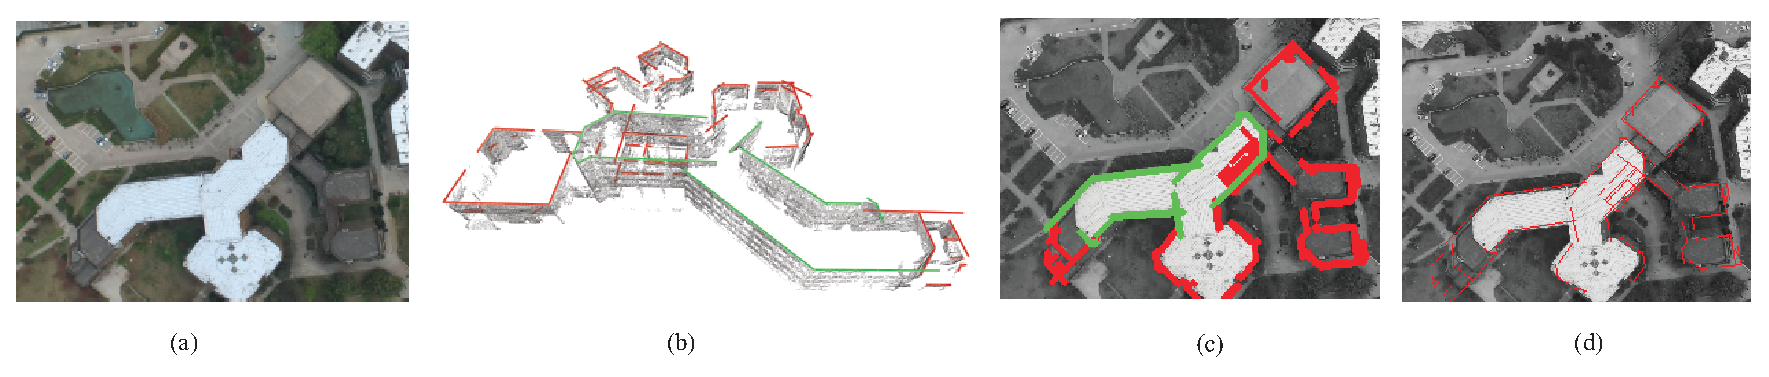
\includegraphics[width=\textwidth]{figures/teaser_eps}
 	\caption{abcd}
 	\label{fig:overview}
 \end{figure*}
 %	
\section{Introduction}
%
As a key technique to image-based navigation, augmented reality (AR) and 3D reconstruction, geo-localization has drawn massive attentions in the literature. When presenting a geo-localization problem, an image or a frame of video is often used as the query data, a 3D model is needed to provide a global coordinate, a sensor prior is optionally employed and the camera pose with respect to the global coordinate system is to be estimated. 

In this work, we estimate the camera pose using an overhead image captured by a low-altitude aerial device as query and a corresponding building point cloud as 3D model. Comparing to existing methods using images captured on the ground or in high-altitude, we are not able to take advantages of vanishing points and suffer from more critical perspective effect. There are two key observations that vertical facades of a point cloud correspond to edges of building roofs in the overhead image and that roofs at different altitudes are of different scales in the image, which inspires us to treat this geo-localization problem as a combination of a multi-layer shape matching problem and a global optimization procedure. 
%利用这个方法,我们可以。。。。。
%
\section{Our Approach}
Given a building point cloud, we first extract contours of building roofs in different altitudes according to the altitude histogram of points, where each contour is fit into a set of line segments (Figure 1b,c). And then the contours are matched with the edge map of the overhead image respectively and achieve a local project matrix for each contour (Figure 1d). To achieve the global project matrix between the whole point cloud and the overhead image, we need a series of pairs of 3D feature points and corresponding 2D feature points. To this end, we use the intersections of neighboring line segments of building roof contours as 3D feature points. 
% For each 3D feature point, we find a corner in the overhead image as its paired 2D feature point in the k*k neighborhood of its corresponding point in the image after shape matching (Figure 2). 
For each 3D feature points, we search the k*k neighborhood of its corresponding point in the overhead image after shape matching, and find a corner as its paired 2D feature point (Figure 2).
With this set of paired 3D and 2D feature points, we can calculate a global project matrix by minimize an energy function based on distance transformation, with which we can finally estimate the 6 DoF camera pose in point cloud coordinate system.
% Be more specific?

Figure 1(e) shows the result of the proposed method by projecting roof contours onto the overhead image. 



	\bibliographystyle{acmsiggraph}
	\bibliography{Alignment_of_Model}
\end{document}

%---------------------- Introduction ---------------------------------
%
